\let\negmedspace\undefined
\let\negthickspace\undefined
\documentclass[journal]{IEEEtran}
\usepackage[a5paper, margin=10mm, onecolumn]{geometry}
%\usepackage{lmodern} % Ensure lmodern is loaded for pdflatex
\usepackage{tfrupee} % Include tfrupee package

\setlength{\headheight}{1cm} % Set the height of the header box
\setlength{\headsep}{0mm}     % Set the distance between the header box and the top of the text
\usepackage{xparse}
\usepackage{gvv-book}
\usepackage{gvv}
\usepackage{cite}
\usepackage{amsmath,amssymb,amsfonts,amsthm}
\usepackage{algorithmic}
\usepackage{graphicx}
\usepackage{textcomp}
\usepackage{xcolor}
\usepackage{txfonts}
\usepackage{listings}
\usepackage{enumitem}
\usepackage{mathtools}
\usepackage{gensymb}
\usepackage{comment}
\usepackage[breaklinks=true]{hyperref}
\usepackage{tkz-euclide} 
\usepackage{listings}
% \usepackage{gvv}                                        
\def\inputGnumericTable{} 
\usepackage[latin1]{inputenc}                                
\usepackage{color}                                            
\usepackage{array}                                            
\usepackage{longtable}                                       
\usepackage{calc}                                             
\usepackage{multirow}                                         
\usepackage{hhline}                                           
\usepackage{ifthen}                                           
\usepackage{lscape}

\begin{document}

\bibliographystyle{IEEEtran}
\vspace{3cm}

\title{7-7.3-5}
\author{EE24BTECH11006 - Arnav Mahishi}
% \maketitle
% \newpage
% \bigskip
{\let\newpage\relax\maketitle}

\renewcommand{\thefigure}{\theenumi}
\renewcommand{\thetable}{\theenumi}
\setlength{\intextsep}{10pt} % Space between text and floats


\numberwithin{equation}{enumi}
\numberwithin{figure}{enumi}
\renewcommand{\thetable}{\theenumi}
Question: If a circle passes through the point $\brak{0,0}$,$\brak{a,0}$,and $\brak{0,b}$ then find the coordinates of its centre.\\
\begin{table}[h!]    
  \centering
  \begin{table}[H]
    \centering
    \begin{tabular}{|c|c|c|c|c|c|c|}
        \hline
        & \multicolumn{4}{c|}{\textbf{DESTINATIONS}} & \textbf{Supply} \\ \cline{2-5}
        \textbf{SOURCES} & P & Q & R & S & \\ \hline
        \textbf{1} & 13 & 8 & 12 & 9 & 20 \\ \hline
        \textbf{2} & 10 & 7 & 5 & 20 & 10 \\ \hline
        \textbf{3} & 3 & 19 & 5 & 12 & 50 \\ \hline
        \textbf{4} & 4 & 9 & 7 & 15 & 30 \\ \hline
        \textbf{5} & 14 & 0 & 1 & 7 & 40 \\ \hline
        \textbf{Demand} & 60 & 10 & 20 & 60 & \\ \hline
    \end{tabular}
\end{table} 

  \caption{Input Parameters}
\end{table}\\
Solution:
\begin{align}
    \text{Given pts $x_1$,$x_2$,$x_3$ on circle: }\myvec{2x_1&2x_2&2x_3\\1&1&1}^T\myvec{u\\f}&=-\myvec{\norm{x_1}^2\\\norm{x_2}^2\\\norm{x_3}^2}\\
    \implies\myvec{2x_1^T&1\\2x_2^T&1\\2x_3^T&1}\myvec{u\\f}&=\myvec{0\\-a^2\\-b^2}\\
    \implies\myvec{0&0&1\\2a&0&1\\0&2b&1}\myvec{u\\f}&=\myvec{0\\-a^2\\-b^2}
\end{align}
The augemented matrix for this
\begin{align}
    \myvec{0&0&1&0\\2a&0&1&-a^2\\0&2b&1&-b^2}\xleftrightarrow[]{R_2 \leftarrow {R_2-R_1}}\myvec{0&0&1&0\\2a&0&0&-a^2\\0&2b&1&-b^2}\\
    \implies\xleftrightarrow[]{R_3 \leftarrow {R_3-R_1}}\myvec{0&0&1&0\\2a&0&0&-a^2\\0&2b&0&-b^2}
\end{align}
Let $u=\myvec{-x\\-y}$ then
\begin{align}
    \myvec{2a&0}u=-a^2\text{ and }\myvec{0&2b}u&=-b^2\\ 
\end{align}
\begin{align}
    \implies\myvec{2a&0}\myvec{-x\\-y}&=-a^2\\
    \implies-2ax=-a^2\implies x&=\frac{a}{2}\\
    \myvec{0&2b}\myvec{-x\\-y}&=-b^2\\
    \implies-2by=-b^2\implies y&=\frac{b}{2}\\
    \implies u=\myvec{-x\\-y}&=-\myvec{\frac{a}{2}\\ \frac{b}{2}}\\
    \therefore c=-u&=\myvec{\frac{a}{2}\\ \frac{b}{2}}
\end{align}
\begin{figure}[h!]
   \centering
   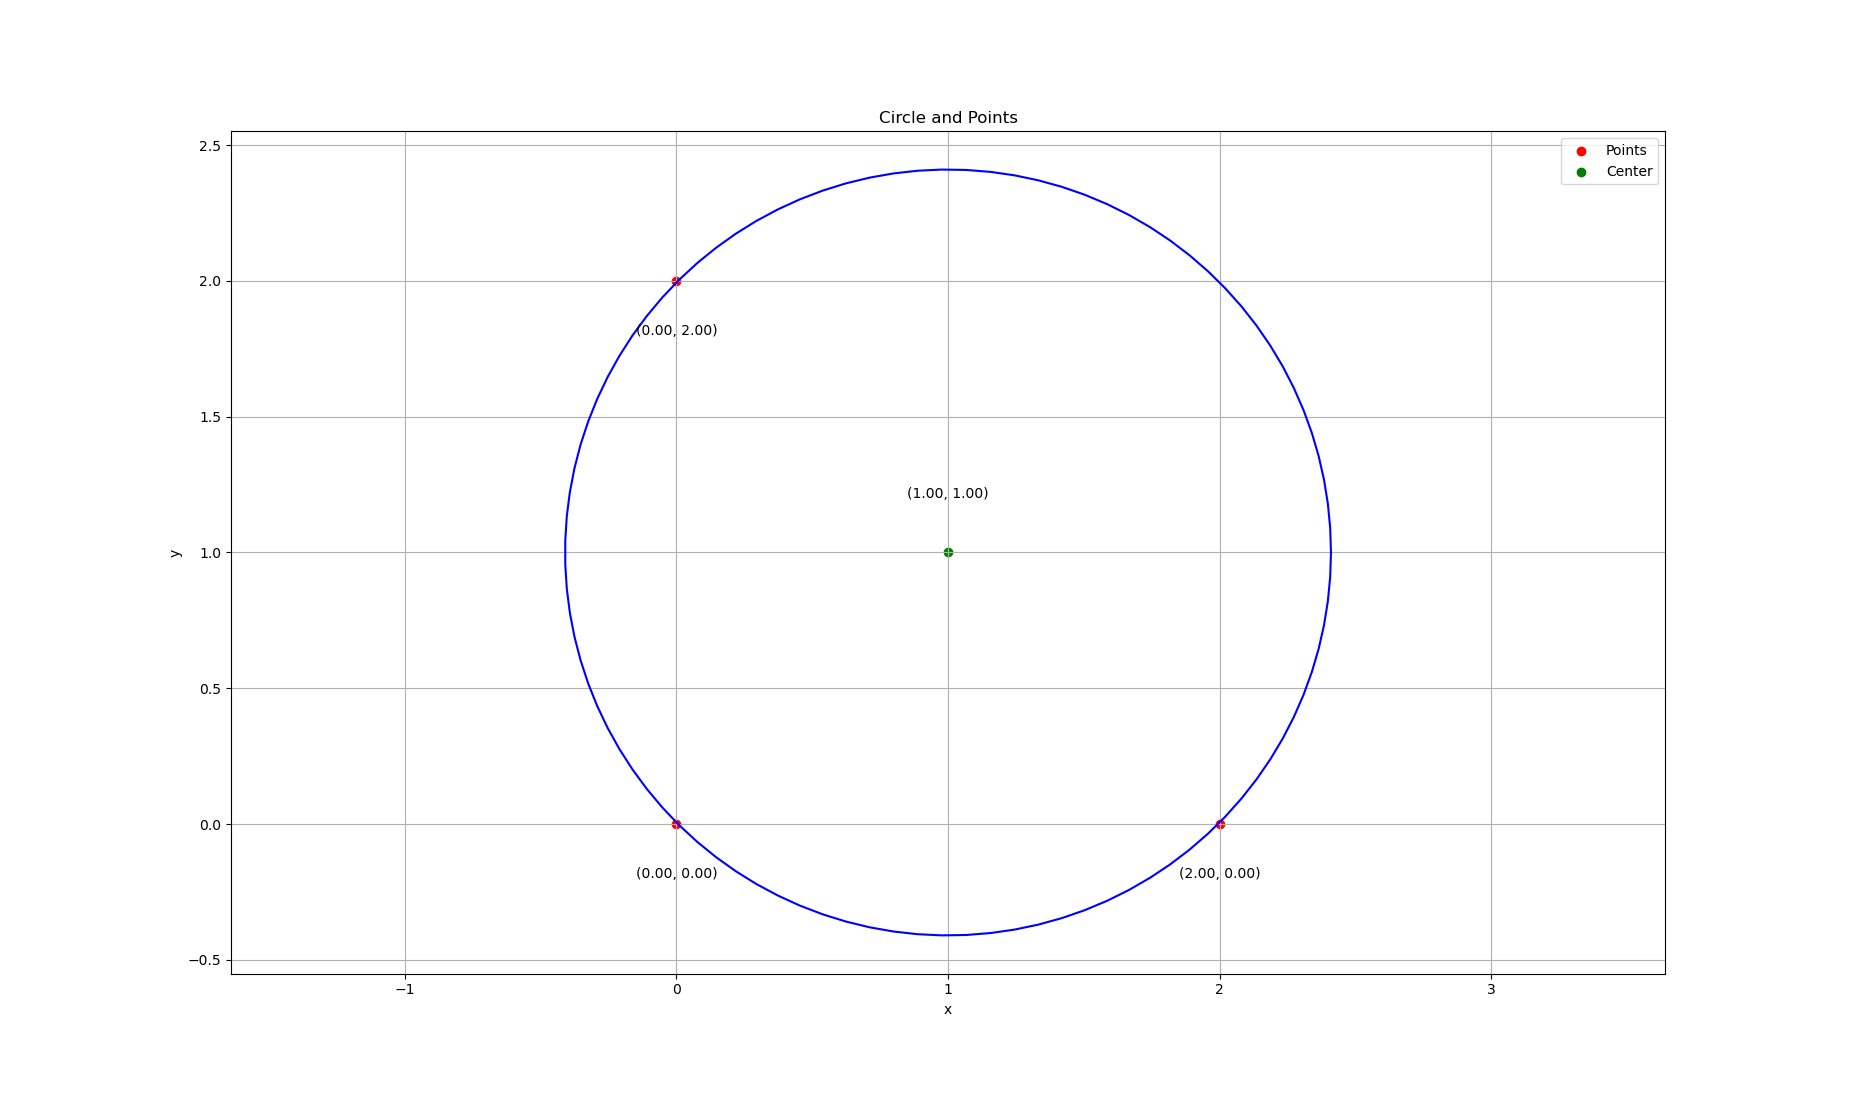
\includegraphics[width=0.7\linewidth]{figs/Figure_1.png}
   \caption{Plot of circle  }
   \label{stemplot}
\end{figure}
\end{document}
